\subsection{Background: compute-optimal and overtrained models}\label{sec:balancing_background}

Given a fixed training FLOPs budget, $C$, how should we allocate model
size $N$ versus number of training tokens $D$ in order to minimize
\emph{loss}?
\citet{hoffmann2022empirical} propose to model loss as:
\begin{equation}\label{eq:chinchilla}
L(N,D) = E + \nconst N^{-\alpha} + \dconst D^{-\beta}
\end{equation}
%
$\nconst$, $\alpha$, $\dconst$, and $\beta$ are parameters fit on
observed training runs.  From \cref{eq:chinchilla},
\citep{hoffmann2022empirical} derives functions for loss-optimal
$\nopt(C)$ and $\dopt(C)$ (constraining $L(N,D)$ by $C \approx 6 N
D$).
%
Results indicate $\nopt$ and $\dopt$ scale roughly equally as $C$
increases, with the optimal $\nicefrac{D}{N}$ ratio relatively
constant at around 20 TPP\@.  Replication studies have found similar
results~\citep{besiroglu2024chinchilla,porian2024resolving},
and 20 TPP has become a rule-of-thumb for compute-optimal
training~\citep{dey2023cerebras,zhang2024how}.
%
%In this work, we call models \emph{undertrained} (or
%\emph{overtrained}) when trained below (or above) 20 TPP\@.

Overtrained, inference-efficient
models~\citep{touvron2023llama,biderman2023pythia,dubey2024llama} have
largely trained with similar batch sizes to those used in
compute-optimal training; such efforts should now consider training
with much greater data parallelism, leveraging our finding that
$\bopt$ and $\bcrit$ will be higher given the higher training $D$.

%Discuss power laws without irreducible loss, e.g. in \citet{kaplan2020scaling}
%
%\begin{equation}\label{eq:powerlaw}
%L(x) = c x^{m}
%\end{equation}

\subsection{Methods: exploring the trade-offs of FLOPs vs.\ time}

%We can use our $\cbs$ power law to help explore the tradeoffs of FLOPs
%vs.\ time in LLM pre-training.
%
%However,
To compare models of different sizes on a common temporal
axis, we must map number-of-optimization-steps to a common temporal scale.
%
Our initial approximation is
%\begin{equation}\label{eq:ttime}
\mbox{$\ttime \propto \nicefrac{\totflopstext}{B}$},
%\end{equation}
which is also FLOPs \emph{per token} times number of steps.  E.g., if
\mbox{$\flops \approx 6ND$}, \mbox{$\ttime \approx {6ND}/{B} = 6N \cdot S$}.  This
aligns well with our measured runtimes: doubling N doubles step time;
doubling B halves wall-clock time (for the same $S$).
%
%Note $\nicefrac{\flops}{B}$
%correlates well with real measurements of our training runs: doubling
%$N$ (and thus $\flops$) makes each step take roughly twice as long,
%while doubling $B$ cuts wall-clock training time in half.}
%Indeed, ``data parallelism can achieve near-perfect scaling at
%small scales''~\citep{smith2022using}.}

Now, assume a model of size $N$ can train to loss $\lhat$ using
$\dmin$ tokens (here \emph{min} denotes using $\bopt$).
%
Let us refer to $N$ and $\dmin$ as a \emph{base setting}.
%
A variety of $N$, $\dmin$ pairs can reach $\lhat$ in the $\bopt$
setting, from small models trained on many tokens, to large models
trained on fewer tokens.  \citet{hoffmann2022empirical}~refers to
these as iso-loss \emph{contours} of \cref{eq:chinchilla}.
%
Suppose a given base setting requires $\minflops$ FLOPs.
%
From this setting, we may increase $B$ to decrease training time
(fewer steps), but \cref{eq:s_extra} indicates a need for $(1 +
{B}/{\cbs})$ extra \emph{data} in order to reach the same $\lhat$.  If
FLOPs is linear in $D$ (as in $C = 6ND$), we will require the same
proportion of extra FLOPs, i.e.,
\begin{equation}\label{eq:flops_extra}
  \totflops = \minflops(1 + {B}/{\cbs(\dmin)})
\end{equation}
where $\totflops$ denotes the total FLOPs needed at $B > \bopt$, and
$\cbs(\dmin)$ captures that the excess FLOPs depends on $\bcrit$,
which itself scales with $\dmin$.  In other words, the base setting
dictates $\bcrit$, and $B/\bcrit$ dictates the excess FLOPs.
%Intuitively, training to $\lhat$ with $B > \bopt$ saves time but costs
%FLOPs.

Consider a target FLOP budget of $\totflops = \hatf$ and the goal of
reaching $\lhat$ \emph{as fast as possible}.
%
Since time $\propto \nicefrac{\totflopstext}{B}$, time is minimized by
maximizing $B$.  However, by construction, $B$ is not a free variable:
it is constrained by \cref{eq:flops_extra} and can be expressed as a
function of $N$ and $\dmin$:
\begin{equation}\label{eq:b_equation}
  B(N,\dmin) = \left(\frac{\hatf}{\minflops} - 1 \right)\cbs(\dmin)
\end{equation}

Time is therefore minimized by finding $N$, $\dmin$ that maximize this
function (over all the $N$, $\dmin$ that train to loss $\lhat$).
%
The ${\hatf}/C$ ratio is a measure of the \emph{excess} FLOPs that can
be spent toward increasing $B$; it is largest when $\minflops$ is
smallest, i.e., when $N$ and $\dmin$ is most compute-efficient (i.e.,
$N/\dmin \approx$ 20~TPP).
%
But \cref{eq:b_equation} as a whole captures an elegant tension
between compute efficiency and $\cbs$: we can maximize $B$ (and
minimize training time) by either
\begin{inparaenum}[(1)]
 \item minimizing the FLOPs of the base setting (generating more
   excess FLOPs for increasing $B$), or
 \item maximizing $\dmin$ (overtraining, which increases $\cbs(\dmin)$).
\end{inparaenum}
%
For a given $\hatf$, either (1) or (2) may take
precedence.
%, depending
%on how compute efficiency and $\cbs$ scale relative to $\dmin$.

We use the following procedure to explore the time vs\@. compute
Pareto frontier for a target loss $\lhat$:
% Our full process for generating FLOPs vs.\ time curves is:
\begin{enumerate}
  \item Fit \cref{eq:chinchilla} on our $\bopt$ training runs.
    Express resulting $L(N,\dmin)$ as ${\dmin}_{\lhat}(N)$.
  \item Using ${\dmin}_{\lhat}(N)$, get contour points $\langle N,
    {\dmin} \rangle$ of the given $\lhat$.
    %
    % D = \left(\frac{\dconst}{\lhat - E - \nconst N^{-\alpha}}\right)^{\frac{1}{\beta}}
    %
    Each such pair consumes $\minflops \approx 6 N \dmin$
    FLOPs and takes $\nicefrac{\minflops}{B}$ time (rightmost points
    on \cref{fig:paretos} curves).
  \item Use \cref{eq:flops_extra} to compute $\totflops$ as we scale
    $B$ (crucially, using the estimate of $\cbs$ from fitted
    \cref{eq:cbs_scaling}), and generate further points along each
    curve.
  \item The non-dominated points over all curves provide the time
    vs.\ compute Pareto frontier.
\end{enumerate}

\subsection{Results: balancing time and compute}

We carry out this procedure using model sizes of 150M, 210M, 550M,
1.1B, and 2.1B, and a loss target of $\lhat$=2.6, yielding iso-loss
contour points from 150M 600TPP to 2.1B 2TPP.  Our fit of
\cref{eq:chinchilla} yielded $\alpha$=$0.313$ $\approx$
$\beta$=$0.282$, giving an optimal TPP ratio of $\approx$20.6 at
$\lhat$=2.6.

\finding{Overtrained, but not undertrained, models are on the FLOPs
  vs.\ time Pareto frontier.}

\begin{figure}[H]
    \centering
    \begin{minipage}{0.33\textwidth}
        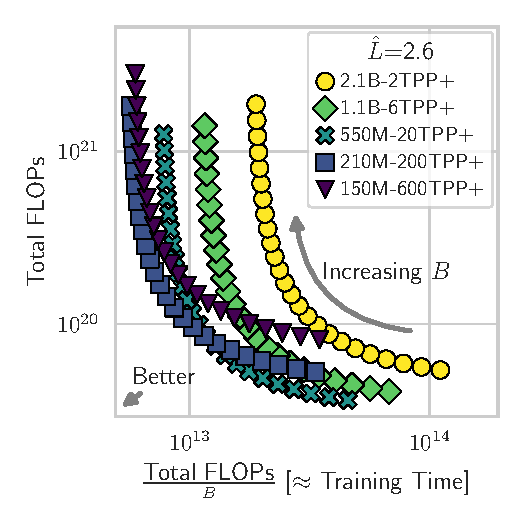
\includegraphics[trim={0.3cm 0.4cm 0.3cm 0.3cm}, clip, width=\linewidth]{pdffigs/pareto.l=2.6.v3.pdf}
    \end{minipage}\hfill
    \begin{minipage}{0.33\textwidth}
        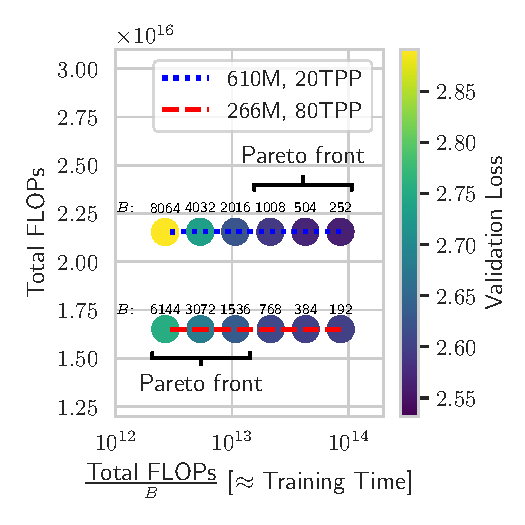
\includegraphics[trim={0.3cm 0.4cm 0.3cm 0.3cm}, clip, width=\linewidth]{pdffigs/loss_data.241005_batchsizes.flop_flops3.pdf}
    \end{minipage}\hfill
    \begin{minipage}{0.33\textwidth}
        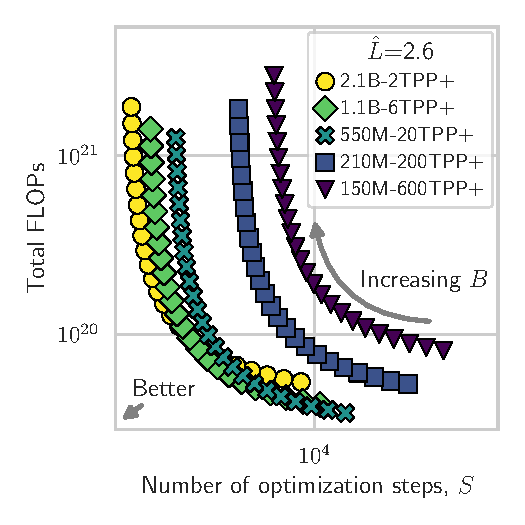
\includegraphics[trim={0.3cm 0.4cm 0.3cm 0.3cm}, clip, width=\linewidth]{pdffigs/pareto.l=2.6.v3.STEPS_ONLY.pdf}
    \end{minipage}
    \caption{($\leftfig$): Iso-loss curves illustrating time--compute
      Pareto frontier ($\lhat$=2.6). As $B$ increases along curves,
      more compute (y-axis), but less time (x-axis) is required. Here
      time $\propto \nicefrac{\totflopstext}{B}$.  ($\middlefig$):
      Observed runs where some overtrained models (red line) are on
      frontier: $L$ in color, $B$ labeled.  ($\rightfig$): Iso-loss
      curves, but where time = steps; a very different frontier
      emerges.\label{fig:paretos}}
\end{figure}


Specifically, when using $\ttime \propto \nicefrac{\totflopstext}{B}$,
we find overtrained models are FLOP-optimal at certain time budgets
(\cref{fig:paretos}, $\leftfig$).  Compute-efficient 20~TPP are
optimal in pure FLOPs (i.e., ignoring time), as expected, while
compute-efficient and overtrained models dominate undertrained ($<$ 20
TPP) models in time and FLOPs.  Indeed, this is expected from
\cref{eq:b_equation}: \emph{under}training reduces both the excess
FLOPs and $\cbs$ terms, and thus is never optimal with this model of
time.
%
%Additional interesting Pareto frontiers are given in
%\cref{sec:pareto_appendix}, including for other fits to
%\cref{eq:chinchilla} (from the literature), other loss targets, and
%other models of training time that account for both data and model
%parallelism.
% Refer to \cref{fig:pareto_steps_only} in
% \cref{sec:pareto_steps_only} for what happens if we consider
% all the FLOPs to be parallelizable, and why that isn't a good idea.

\finding{When using $B \gg \bopt$, it is Pareto-inefficient to train to 20~TPP.\label{finding:largeb}}

%We now discuss a somewhat subtle matter that has a very clear and
%important conclusion.

Notice that \cref{fig:paretos} adds ``\emph{$\ldots$TPP+}'' to curve
labels.  Here the $+$ sign is a reminder that as we increase $B$, we
require $(1 + {B}/{\cbs})$ \emph{extra data} to reach the
same $\lhat$; i.e., points with higher $B$ are trained to a higher
\emph{actual TPP} than the base setting.
%at $\tpp$=$\nicefrac{\dmin}{N}$.
For example, once the 2TPP+ curve in \cref{fig:paretos} reaches
10$\times$ its minimum FLOPs, it is \emph{actually} training at 20
TPP\@.
%
Since starting from an undertrained base setting is never Pareto
optimal (as just discussed above), \emph{it is \textbf{always}
suboptimal to train a model with a large $B$ to 20 actual TPP}.  If
large-batch training is needed, the configuration should start from a
20 TPP+ base setting and scale $B$ from there (to $>$20 TPP).

We can see this finding play out in real training runs.
\cref{fig:paretos} (middle) demonstrates observed runs where our 266M
80TPP models \emph{dominate} our 610M 20TPP models (i.e., in FLOPs
\emph{and} time)---when both train with large $B$.  (Note in this
plot, results are not iso-loss: the frontier is over $L$, $C$, and
time.)

\finding{The Pareto-optimal settings depend on the formulation of
  time/parallelism strategy.}

While $\nicefrac{\text{FLOPs}}{B}$ is a good model of data parallel
training, it does not incorporate the potential for model
parallelism~\citep{smith2022using}.
%
In the extreme we could assume that all $6N$ FLOPs could be executed
concurrently per input token.  Under this formulation, training time
is proportional only to the number of steps, regardless of model
scale.
%
\cref{fig:paretos} ($\rightfig$) shows the Pareto frontier that would
result from this formulation; if we pay no time cost for larger
models, we can train faster by using undertrained large models,
although, exactly as with overtrained models, they suffer in FLOPs.

While LLMs cannot be fully parallelized due to the inherent sequential
nature of a Transformer's layer-by-layer computation, this formulation
could be refined by incorporating depth or other architectural
features.
%
For example, \citet{inbar2024time} predict training time via linear
regression over total FLOPs and memory-copy operations, fit to real
(single-TPU) runs.
%
As formulations improve, different Pareto-optimal configurations will emerge.

\finding{Inaccurate $\bcrit$ scaling leads to inaccurate
  Pareto-optimal configurations.}

Because the Pareto frontier in \cref{sec:balancing} depends directly
on the $\bcrit$ power-law fit, any error in that fit produces
corresponding errors in the predicted trade-offs between training time
and compute.  Accurate $\bcrit$ estimation, in turn, depends on
effective $\lambda$ tuning
(\cref{finding:wd_bopt,sec:app_wd_affects_b}).  When $\lambda$ is
fixed as in standard practice (and thus the $\bcrit(D)$ slope is
misestimated), $\bcrit$ will be systematically over- or underpredicted
at scale, altering the computed frontier and the apparent
Pareto-optimal configurations.
%
To illustrate, artificially varying the $\bcrit$ exponent changes
which models appear on the frontier: as the exponent increases (and
$\bcrit$ rises), higher-TPP models move to the frontier; when $\bcrit$
is underestimated, only low-TPP (e.g., 20~TPP) models appear
Pareto-optimal.  Hence, an inaccurate $\bcrit$ scaling law produces
misleading frontiers and can lead to unexpectedly-longer training
durations and suboptimal compute allocations.

Recent work suggests that other estimators of $\bcrit$ (such as those
based on the gradient noise scale~\citep{mccandlish2018empirical}) can
also be systematically biased (\cref{sec:app_bcrit}), leading to
similar distortions in the Pareto frontier.

\takeaway{To balance time and compute at a target loss, select $(N,
  D_{\min})$ from \cref{eq:chinchilla}, determine $\bcrit(D_{\min})$
  via \cref{eq:cbs_scaling}, and use \cref{eq:flops_extra} to estimate
  compute for any $B$.  Under $\text{Time}\!\propto\!\text{FLOPs}/B$,
  the resulting time--compute trade-off favors higher $D$
  (overtraining) (\cref{fig:paretos}).}
